\section{Testing}
In der Python Standard Library gibt es das Unit Testing Framework \textbf{unittest}, das erlaubt Unit Tests zu implementieren. 
Django's Unit Tests basieren auf dieser Library und erweitern diese, beispielsweise erbt \textbf{django.test.TestCase} von \textbf{unittest.TestCase}. Weiter werden auch Integrationtests ermöglicht.

\subsubsection{Beispiel Integrationtests}
\begin{python}
from django.test import Client, TestCase
from django.contrib.auth.models import User

class AboutViewsTests(TestCase):

   def setUp(self):
       self.user = User.objects.create(username='testuser')
       self.user.set_password('12345')
       self.user.save()
       self.client = Client()
       self.client.login(username='testuser', password='12345')

   def test_about_get(self):
       response = self.client.get('/about/')
       self.assertEquals(response.status_code, 200)      
\end{python}

\subsection{Continuous Integration (CI)}
Der Aufbau der Continuous Integration Umgebung des strongMans ist nicht trivial und stellt folgede Anforderungen:
\begin{itemize}
	\item Aufbau von IPsec Tunnels zwischen mindesten zwei Rechnern
	\item automatisierter Ablauf
	\item geringe Einarbeitungszeit in Technologien
	\item möglichst kostenfreie Dienste nutzen
\end{itemize}
Um den Anforderungen gerecht zu werden setzten wir auf ein Zusammenspiel folgender Tools:
\paragraph{GitHub} wird von uns als online Repository verwendet und wird mit dem Versionsverwaltungssystem Git eingesetzt. Weiter bietet es für andere Dienste WebHooks an. 
\paragraph{Travis CI} wird als eigentlicher Continuous Integration Anbieter verwendet. Es ermöglicht automatisierte Builds und Tests. Travis CI ist für Projekte, welche auf GitHub gehostet werden, ausgelegt.

\paragraph{Docker} Um die strongSwan Konfiguration direkt zu testen, wird docker-compose eingesetzt. Docker-compose gewährleistet mehrere Docker Container zu builden, ein Netzwerk untereinander und somit einen IPsec Tunnel aufzubauen. \\

\subsubsection{Ablauf}
\begin{figure}[H]
\centering
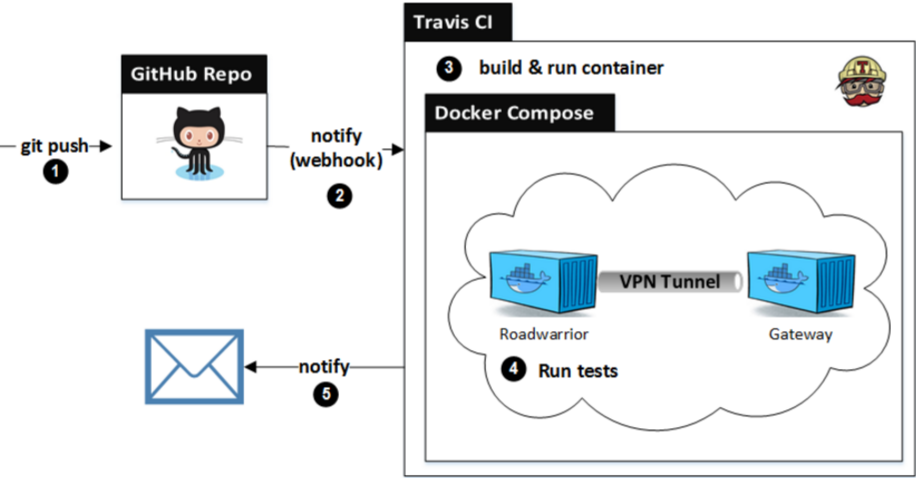
\includegraphics[width=420pt]{images/testing.png}
\caption[Schematische Darstellung der Testumgebung]{Schematische Darstellung der Testumgebung}
\end{figure}\medskip
\begin{enumerate}
	\item git push, lokaler Code wird auf GitHub publiziert.
	\item Travis CI wird durch WebHook notifiziert.
	\item Travis CI buildet zwei Docker Container, welche auf der Basis des offiziellen Django Container aufbaut.
	\begin{enumerate}
         \item StrongSwan mit den nötigen Plugins wird installiert und gestartet.
         \item Auf dem Roadwarrior wird die strongMan Applikation vom GitHub Repository installiert und der aktuelle Branch wird eingecheckt.
      \end{enumerate}
      \item Der Roadwarrior started die Unit- und die Integrationstests. Dabei werden zwischen den Docker Container diverse Ipsec Tunnels auf- und abgebaut.
      \item Erfolg und Misserfolg ist auf der ReadMe Seite auf Github einsehbar.
\end{enumerate}

\newpage
\subsection{Usability Tests}

Die Usability Tests sollen Ablauffehler aufzeigen und die Benutzbarkeit der Applikation insgesamt steigern. Dazu sind in einer ersten Phase zwei Personas erstellt worden.
\\
\decision{Usability Tests vs. Server Features}
\label{UsabilityEntscheid}
Am Ende der zweit letzten Construction Phase, nach einer Besprechung mit Herrn Steffen, entschieden wir uns Usability Tests durchzuführen und den Server Teil der Applikation in diesem Projekt nicht zu implementieren.
Damit werden die Use Cases UC03: Child\_SA beenden und UC06: Admin Mode wechseln hinfällig.

\subsubsection{Primäre Persona User}





\noindent\begin{minipage}[t]{0.5\textwidth}
\vspace{0pt}
    \begin{tabular}{ l l }
        Name: & Markus Egger \\
        Alter: & 40 Jahre \\
        Beruf: & Verkäufer Aussendienst \\
        Wohnort: & Uster ZH \\
        Zivilstand: & Verheiratet, 2 Kinder \\
        Hobbies: & Gleitschirm, Bowling \\
        Sprachen: & Deutsch / Englisch \\
    \end{tabular}
\end{minipage}
\hfill
\begin{minipage}[t]{0.5\textwidth}
\vspace{0pt}

\begin{figure}[H]
\centering
    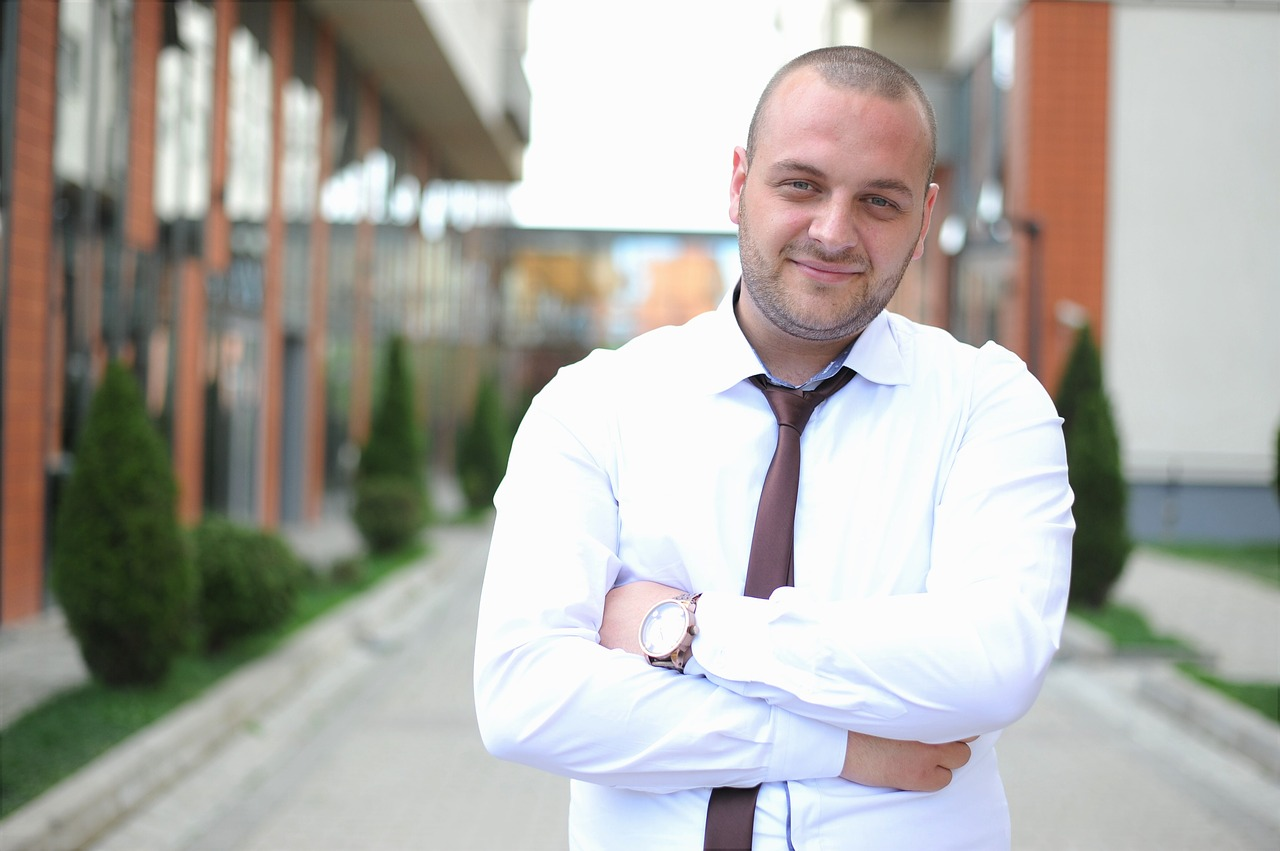
\includegraphics[width=230px]{images/persona_business.jpg}
    \caption[Primäre Persona User]{Primäre Persona User}
\end{figure}
\end{minipage}
\medskip


Markus Egger arbeitet in einem mittelgrossen Industrieunternehmen und verkauft dort Isolationsmatten aus Steinwolle. Da er viel auf Reisen bei seinen Kunden ist und dadurch längere Zeit keinen physischen Zugang zum Firmennetzwerk hat, benutzt er eine VPN Software um auf firmeninterne Daten zuzugreifen. Seine Informatikfähigkeiten beziehen sich dabei auf die in seiner KV Lehre erworbenen Kenntnisse mit Email, Word und Excel, sowie dem oberflächlichen Umgang mit ERP/CRM Systemen.
Markus beherrscht die englische Sprache auf Verhandlungsniveau.

Zusätzlich zu seinen Reisen arbeitet Markus gerne auch mal Zuhause, um mehr Zeit bei seinen erst kürzlich eingeschulten Kindern zu verbringen und seine Frau zu entlasten.

\subsubsection{Test Vorlage}


Sie sind Angestellter in der Personalabteilung der Industriefirma Techtronic AG und arbeiten heute zum ersten Mal Zuhause an ihrem Arbeitslaptop. Um Zugriff auf firmeninterne Dokumente zur erhalten, müssen Sie eine sichere Verbindung zur Tectronic AG aufbauen. Dazu hat Ihnen die Informatikabteilung ein USB-Stick mit Anleitungen, Username, Passwort und Zertifikatsdateien zur Verfügung gestellt. Ihre Aufgabe ist es nun, die unten aufgeführten Tasks zu lösen.

\paragraph{Passwort ändern}
Loggen Sie sich ein und ändern Sie ihr Passwort. \\


\begin{tabular}{ | p{0.14\textwidth} | p{0.77\textwidth} | }
\hline
Preconditions: & Applikation ist gestartet. User befindet sich auf der Login Seite. \\
\hline
Hilfsmittel: & Username und aktuelles Passwort \\
\hline
Artefakte: & User konnte sich einloggen. \\ 
& Passwort ändern Feld gefunden. \\
& Passwort konnte geändert werden. \\
\hline
\end{tabular}

\paragraph{Verbindung erstellen}
Erstellen Sie eine neue Verbindung zur HSR mit den gegebenen Daten. \\


\begin{tabular}{ | p{0.14\textwidth} | p{0.77\textwidth} | }
\hline
Preconditions: & User befindet sich eingeloggt auf der Startseite von strongMan. Connections und Certificates sind leer. Der System Administrator hat eine Anleitung zum Erstellen der Verbindung zur Verfügung gestellt. \\
\hline
Hilfsmittel: & Schritt für Schritt Anleitung mit Server, Username, Passwort, CA-Zertifikat, Identity \\
\hline
Artefakte: & User hat den Connections Bereich gefunden. \\
& User hat den Add Button gefunden. \\
& Der richtige Authentifizierungstyp ist ausgewählt. \\
& Verbindung richtig ausgefüllt und erstellt. \\
\hline
\end{tabular}


\paragraph{Verbindung starten / stoppen}
Starten Sie die Verbindung und stoppen Sie diese wieder. \\


\begin{tabular}{ | p{0.14\textwidth} | p{0.77\textwidth} | }
\hline
Preconditions: & User befindet sich auf der Connections Seite. Die in Aufgabe 2 erstellte Connection ist abgespeichert. \\
\hline
Hilfsmittel: & - \\
\hline
Artefakte: & User erkennt den On/Off Button. \\
& User kann die Verbindung starten. \\
& User ist sich bewusst, dass die Verbindung jetzt steht (Fragen!). \\
& Verbindung ist wieder gestoppt. \\
\hline
\end{tabular}

\newpage
\subsubsection{Sekundäre Persona Administrator}

\noindent\begin{minipage}[t]{0.5\textwidth}
\vspace{0pt}
    \begin{tabular}{ l l }
        Name: & Remo Stoop \\
        Alter: & 28 Jahre \\
        Beruf: & System Administrator \\
        Wohnort: & Greifensee ZH \\
        Zivilstand: & Konkubinat, 1 Kind \\
        Hobbies: & Raspberry Pi, Gamen \\
        Sprachen: & Deutsch / Englisch \\
    \end{tabular}
\end{minipage}
\hfill
\begin{minipage}[t]{0.5\textwidth}
\vspace{0pt}
\begin{figure}[H]
\centering
    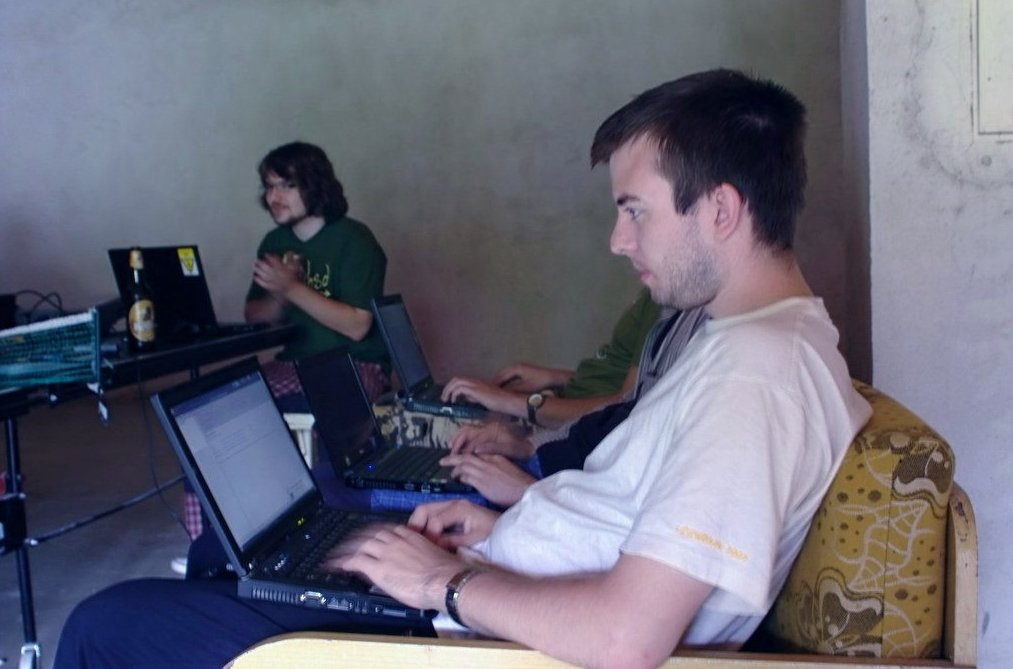
\includegraphics[width=230px]{images/administrator.jpg}
    \caption[Sekundäre Persona Administrator]{Sekundäre Persona Administrator}
\end{figure}
\end{minipage}
\medskip

Remo Stoop arbeitet wie Markus Egger im gleichen mittelgrossen Industrieunternehmen, welche Isolationsmatten herstellt. Er ist dort als System Administrator angestellt und verantwortlich für die Netzwerkinfrastruktur und der Netzwerksicherheit, inklusive dem Netzwerkzugriff von aussen.  Remo hat sich bewusst in Richtig Netzwerk weitergebildet. Nach seiner Lehre als Informatiker Systemtechnik hat er zwei fünf tägige Cisco Netzwerk Kurse besucht und ist seit dem netzwerktechnisch auf dem neusten Stand. Die symmetrischen und asymmetrischen Verschlüsslungstechniken kennt er oberflächlich aus einem Modul aus seiner Lehre.

Auch Remo arbeitet gerne einen Tag in der Woche zuhause, sofern es seine Arbeit erlaubt. Neben seiner Familie ist seine Hauptbeschäftigung das Gamen mit Freunden sowie Raspberry Pi Bastelprojekte.


\subsubsection{Test Vorlage (erweitert User Tests)}

Sie sind Systemadministrator der Industriefirma Techtronic AG und haben zuvor einen strongSwan VPN Server eingerichtet. Nun soll das erste Mal eine Verbindung von ausserhalb (genauer von Ihnen zuhause) in die Firma aufgebaut werden. Dazu stehen Ihnen Username, Passwort und Zertifikatsdateien zur Verfügung gestellt. Ihre Aufgabe ist es nun, die unten aufgeführten Tasks zu lösen.

\paragraph{Key Container hinzufügen}
\begin{enumerate}
    \item Fügen Sie in der Zertifikatsverwaltung einen verschlüsselten PKCS12 Container hinzu.
    \item Fügen Sie in der Zertifikatsverwaltung ein neues Zertifikat mit Private Key hinzu.
    \item Welche Email Adresse ist beim Zertifkat roadwarrior.hsr.ch eingetragen?
    \item Zertifkat roadwarrior.hsr.ch löschen.
\end{enumerate}


\begin{tabular}{ | p{0.14\textwidth} | p{0.77\textwidth} | }
\hline
Preconditions: & User befindet sich auf der Startseite von strongMan. \\
\hline
Hilfsmittel: & Roadwarrior PKCS12 Container mit Passwort, Zertifikat mit Private Key \\
\hline
Artefakte: & User hat den Add Button gefunden. \\
& User konnte den verschlüsselten PKCS12 Container hinzufügen. \\
& User konnte das Zertifikat hinzufügen. \\
& User konnte den Private Key hinzufügen. \\
& User findet Email-Adresse. \\
& User konnte Zertifikat löschen. \\
\hline
\end{tabular}


\subsubsection{Fazit}
Wir haben die Usability Tests mit vier Personen durchgeführt. Die Administrator Tests haben zwei unbeteiligte HSR Studenten durchgeführt und die User Tests zwei User mit Büroerfahrung.

Die wichtigsten Erkenntnisse aus den Tests sind:
\begin{itemize}
    \item Es braucht ein Text, der beschreibt, dass zuerst das Zertifikat und erst danach der Private Key geuploaded werden kann.
    \item Die State Spalte in der Connection Table ist nicht sortierbar.
    \item Der Verbindungstyp muss änderbar sein nach der Auswahl.
    \item Zertifikate müssen in der Verbindungskonfiguration hinzugefügt werden können.
    \item Beschriftung der Remove Buttons muss eindeutig sein. Private Key löscht keine Zertifikate.
    \item Verbindung darf nicht löschbar sein, wenn sie aktiv ist.
    \item Diverese Verbesserungen an der Englischen Sprache sind nötig.
    \item Die Anordnung der Buttons im Add-Certificate Formular verwirrt.
    \item About Pages zeigt keine Infos.
\end{itemize}
